\documentclass[12pt,a4paper]{article}

%\usepackage[lmargin=1.9cm, rmargin=1.9cm,tmargin=1.9cm,bmargin=1.9cm]{geometry}
\usepackage[T1]{fontenc}
\usepackage[utf8]{inputenc}
\usepackage[polish]{babel}
\usepackage{listings}
\usepackage{graphicx}
\usepackage{color}
\usepackage{hyperref}


\newcommand{\HRule}{\rule{\linewidth}{0.5mm}}

% Definicja kodu
\lstset{
	language=Java,
    basicstyle=\footnotesize \ttfamily,
    showstringspaces=false,
    numbers=left,       % where to put the line-numbers
	numberstyle=\tiny,
    tabsize=2,
    inputencoding=utf8,
    extendedchars=\true,
    breaklines=true,
    frame=single
}

\begin{document}

\begin{titlepage}

  \begin{center}
    % Logo
    
\includegraphics[width=0.3\textwidth]{img/logo.jpg}\\[1cm]
    
    % University
    \textsc{\LARGE Wydział Elektryczny \\ Politechniki Warszawskiej}\\[1.5cm]
    
    % Course
    \large \textsc{Algorytm i Struktury Danych -- \\ Projekt indywidualny}\\[0.5cm]

    % Title
    \HRule \\[0.4cm]
    {\huge \bfseries Scheduler }\\[0.2cm]
    \HRule \\[1.5cm]
   
    % Author
    {\large
    Mateusz \textsc{Cieciura} \\ GR1, 234337}
    
    \vfill

    % Date
    {\large \today}
  \end{center}

\end{titlepage}

\tableofcontents

\section{Wprowadzenie}

Zadaniem w projekcie indywidualnym było stworzenie modułu do zarządzania kolejką priorytetową elementów o nazwie \texttt{Jobs}, które posiadają następujące cechy:

\begin{itemize}
	\item identyfikator,
	\item priorytet.
\end{itemize}

Funkcjonalność kolejki priorytetowej można określić np. poprzez interface w języku \texttt{Java}:

\begin{lstlisting}[caption=Interface kolejki priorytetowej]
public interface SchedulerData {
    public void add(Job a); 
    // adds a job to the scheduler    
    public Job remove(); 
    // removes from the scheduler job with the greatest priority
    public boolean changePriority(int id, int priority); 
    // changes priority in particular job, returns false if such job wasn't found
    public boolean isEmpty(); 
    // return true if scheduler has no jobs
}
\end{lstlisting}

\section{Funkcjonalność}

Moduł powinien udostępniac funkcjonalność zarządzania schedulerem komendami zewnętrznymi. Możliwe powinno być: dodawanie i usuwanie elementów oraz zmiana priorytetu istniejącego zadania.

\begin{lstlisting}[caption=Przykładowa sesja modułu]
$ ./sheduler
> jobpush 1 100
> jobpush 2 102
> jobpush 3 103
> jobchange 1 10
> jobpush 4 200
> jobpush 5 10
> jobpush 6 20
> jobchange 2 300
> jobpop
< Job 2
> jobpop
> Job 4
> jobpop
< Job 3
\end{lstlisting}

Dane wyjściowe są wyprowadzane na takie samo wyjście, jak dane wejściowe, tj. jeśli wczytano polecenia z pliku powstanie plik wynikowy ze statystyką przeprowadzonych operacji, jeśli wpisano je z klawiatury to zostaną one wyświetlone na wyjście standardowe.

\section{Główna struktura danych}

Podstawowym zagadnieniem było wybranie struktury danych do przechowywania elementów. Musi ona spewniać pewne kryteria:

\begin{itemize}
	\item wydajność przy dużej liczbie elementów,
	\item szybki dostęp do największego elementu.
\end{itemize}

Po zapoznaniu się z informacjami na temat kolejek priorytetowych wybór padł na \textit{kopiec binarny} (ang. binary heap).

\subsection{Charakterystyka kopca}

Kopiec jest to specjalny rodzaj drzewa binarnego, w którym wartości węzłow dzieci danego są w stałej relacji z wartością rodzica (na przykład wartość rodzica jest większa niż wartości jego dzieci).

\begin{figure}[h]
	\centering
	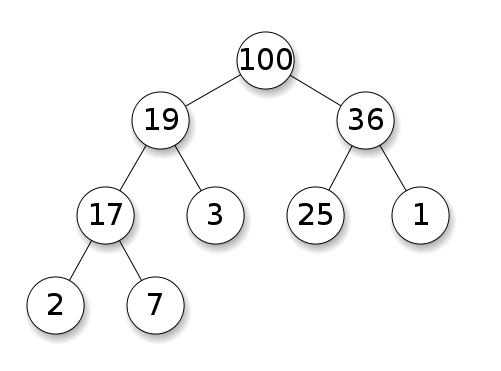
\includegraphics[scale=0.5]{img/heap.png} 
	\caption{Przykład kopca binarnego}
\end{figure}

Jak widać na powyższym rysunku taka struktura danych doskonale nadaje się do przechowywania kolejki priorytetowej, ponieważ największy element jest wyróżniony -- znajduje się w korzeniu kopca.

\subsection{Własność budowy kopca}

Kopiec binarny ma pewną własność, co do jego budowy. Z prawej strony ma niesymetryczną, niepełną budowę. Wiąże się z tym charakterystyka operacji przeprowadzanych na nim.

Gdy dodajemy element, wstawiamy go na sam koniec (podłączamy jako dziecko ostatniego rodzica, które nie ma dwójki dzieci). Natomiast, gdy usuwamy element przesuwamy ostatni element na pierwsze miejsce. W obu przypadkach następnie wykonywane są zamiany elementów, aby przywrócić relację między rodzicami i ich dziećmi.

\subsection{Operacje na kopcu}

\subsubsection{Dodawanie elementu do kopca}

\begin{lstlisting}[caption=Pseudokod algorytmu dodawania elementów do kopca]
funkcja Insert(a):
    size := size + 1
    child := size
    H[child] := a
    dopoki child > 1 oraz H[child] > H[child/2], wykonuj
            zamien miejscami H[child] oraz H[child/2]
            child := child / 2
\end{lstlisting}

\subsubsection{Usuwanie elementu z kopca}

Algorytm prezentuje się następująco:

\begin{enumerate}
	\item usuń wierzchołek ze szczytu kopca,
	\item przestaw ostatni wierzchołek z pozycji n na szczyt kopca; niech k oznacza jego klucz,
	\item spychaj przestawiony wierzchołek w dół, zamieniając pozycjami z większymi z dzieci, aż do przywrócenia warunku kopca (czyli aż dzieci będą mniejsze od k lub element dotrze na spód kopca).
\end{enumerate}

\subsection{Implementacja kopca binarnego}

\textit{Kopiec binarny} implementowany jest za pomocą tablicy elementów. Opisują ją dwa parametry: 

\begin{description}
	\item [\texttt{length}] przechowuje informacje o wielkości całej tablicy, 
	\item [\texttt{heap-size}] przechowuje informacje o ilości elementów. 
\end{description}

Korzeń drzewa przechowywany jest zawsze w pierwszej komórce tablicy. 

Przykład przechowywania kopca binarnego w tablicy:

\vspace{5pt}
\begin{tabular}{| c | c | c | c | c | c | c | c | c | c | c | c | }
	\hline
	\textbf{Indeks tablicy} & 0 & 1 & 2 & 3 & 4 & 5 & 6 & 7 & 8 & 9	\\
	\hline
	\textbf{Wartość komórki} & 20	& 16 & 8 & 10 & 1 5 & 2 & 5 & 7 & 6 & 3 \\
	\hline
	\end{tabular}
\vspace{5pt}

W pierwszej komórce tablicy znajduje się korzeń. Indeksy lewego i prawego dziecka węzła \textit{i} to odpowiedno
 \textit{$2*i+1$} oraz \textit{$2i+2$}. Indeks rodzica węzła to \textit{$\frac{(i-1)}{2}$}.

\section{Implementacja modułu Scheduler}

\subsection{Wprowadzenie}

\begin{figure}[h]
	\centering
	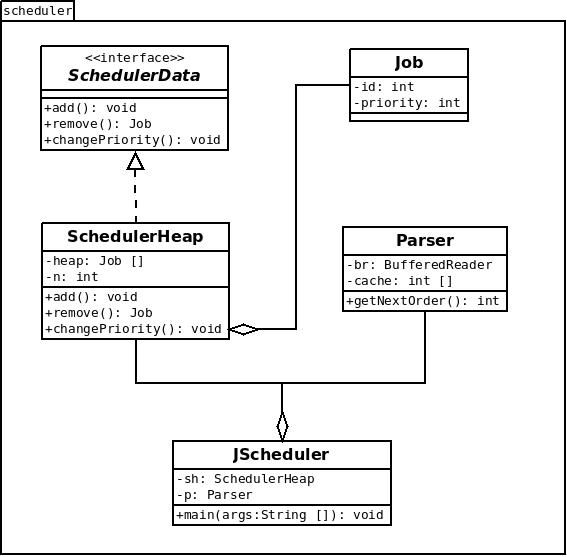
\includegraphics[scale=0.5]{img/diagram.jpg} 
	\caption{Diagram UML modułu JScheduler}
\end{figure}

Wydzialono następujące klasy:

\begin{description}
	\item [Job.java] klasa, która przechowuje pojedyncze zadanie. Posiada pola \texttt{id} oraz \texttt{priority} oraz metody dostępowe
	\item [SchedulerData.java] interfejs reprezentujący kolejkę priorytetową. Posiada operacje \texttt{add()}, \texttt{remove()} oraz \texttt{changePriority()}
	\item [SchedulerHeap.java] klasa implementuje interfejs SchedulerData w postaci kopca binarnego
	\item [JScheduler.java] główna klasa modułu, która wykorzystując w/w klasy zarządza schedulerem
\end{description}

\subsection{Szczegóły implementacji}

\subsubsection{Operacje na kopcu}

Do poprawiania relacji w kopcu służą dwie metody z klasy \texttt{SchedulerHeap}: \texttt{heapUp()} oraz \texttt{heapDown()}.

Po dodaniu elementu wykorzystywana jest pierwsza z nich:

\begin{lstlisting}
    private void heapUp() {
        for (int i = n; i > 0; i--) {
            if (heap[i].getPriority() > heap[(i-1)/2].getPriority()) {
                this.swap(i, (i-1)/2);
            }
        }
    }
\end{lstlisting}

Natomiast po usunięciu elementu i zmianie priorytetu druga z nich:

\begin{lstlisting}
    private void heapDown() {
        int i = 0;
        while (2 * i + 1 < n) { // until there's at least one child
            if (2 * i + 2 >= n) { // if there's only one child
                if (heap[i].getPriority() < heap[2*i+1].getPriority()) { // if child is greater than parent
                    swap(i, 2*i+1);
                    i = 2*i + 1;
                } else {
                    i++;
                }
            } else // there's both children
            if (heap[i].getPriority() < heap[2*i+1].getPriority() || heap[i].getPriority() < heap[2*i+2].getPriority()) {
							// jedno z dzieci jest wieksze od rodzica
                if (heap[2*i+1].getPriority() > heap[2*i+2].getPriority()) {  // left child > right child
                    swap(i, 2*i+1);
                    i = 2*i+1;
                } else { // right child > left child
                    swap(i, 2*i+2);
                    i = 2*i+2;
                }
            } else {
                i++;
            }
        }
    }
\end{lstlisting}


\section{Testy}

Ze względu na charakter testów można podzielić je na dwie kategorie:

\begin{itemize}
	\item testy interaktywne
	\item testy dla badań statystycznych
\end{itemize}

W pierwszym przypadku jest to zbiór testów, które sprawdzają, jak działa program w aspekcie opisanym w funkcjonalności. To znaczy wczytywane są plik z rozkazami lub są wprowadzane one z klawiatury, a następnie moduł generuje pliki wynikowe. W plikach tych znajdują się logi zdjętych zadań w postaci:

\begin{lstlisting}
Popped job (id: 3 priority: 711)
\end{lstlisting}

Oraz informacje o niepowodzeniach przy zmianie priorytetu:

\begin{lstlisting}
Priority not changed. There's no element with such ID!
\end{lstlisting}

Na końcu znajdują się dane dot. obecnej struktury schedulera (po wykonaniu wszystkich zadań) oraz podsumowanie wszystkich operacji:

\begin{lstlisting}
# Jobs left after all operations
# Number of elements: 1
id: 99, priority: 561 

##### Stats ######
# Pushed jobs: 28
# Popped jobs: 28
# Changed jobs: 42
##################
\end{lstlisting}

\subsection{Tryb normalny}

Zgodnie z komunikatami wyświetlanymi przez program, aby uruchomić program należy posłużyć się następującą składanią:

\begin{lstlisting}[caption=Opis wywołania progamu]
java -cp src/ scheduler.JScheduler [-f <file_with_orders>]
\end{lstlisting}

z poziomu katalogu \texttt{.../JScheduler/}.

Jak widać, opcja \texttt{-f} jest opcjonalna. Po zatwierdzeniu polecenia bez niej wchodzimy w tryb interaktywny:

\begin{lstlisting}[caption=Przykład wywołania progamu w trybie interaktywnym]
# Reading from Standard Input
jobpush 1 10
jobpush 2 20
jobpush 3 30 
jobchange 1 100
jobpop
Popped job (id: 1 priority: 100)
jobpop
Popped job (id: 3 priority: 30)
jobpop
Popped job (id: 2 priority: 20)
jobpop
No more jobs. There's nothing to be popped.
# Jobs left after all operations
# Number of elements: 0
##### Stats ######
# Pushed jobs: 3
# Popped jobs: 4
# Changed jobs: 1
##################
\end{lstlisting}

\begin{lstlisting}[caption=Przykład wywołania progamu z plikiem wejściowym]
java -cp src/ scheduler.JScheduler -f test/test3]
\end{lstlisting}

Plik wejściowy ma następującą budowę:

\begin{lstlisting}[caption=Plik testowy test3]
jobpush 1 10
jobpush 2 20
jobpush 3 30
jobpush 4 40
jobpush 5 50
jobpush 6 60
jobpush 7 70
jobpush 8 80
jobpush 9 90
jobpush 10 100
jobpop 
\end{lstlisting}

Po wykonaniu się programu logi zostały zapisane w pliku \texttt{log-jscheduler-13.01.13-17:43:51}. Jego zawartość jest następująca:

\begin{lstlisting}[caption=Zawartość pliku wynikowego]
Popped job (id: 10 priority: 100)
# Jobs left after all operations
# Number of elements: 9
id: 9, priority: 90
id: 8, priority: 80
id: 6, priority: 60
id: 7, priority: 70
id: 3, priority: 30
id: 2, priority: 20
id: 5, priority: 50
id: 1, priority: 10
id: 4, priority: 40

##### Stats ######
# Pushed jobs: 10
# Popped jobs: 1
# Changed jobs: 0
##################
\end{lstlisting}

\subsection{Tryb zbierania statystyk}

W tym trybie za pomocą specjalnej klasy \texttt{StatsGenerator.java} przygotowano wyniki do statystyk.
Stworzono kopce o wielkości 10, 100, 1 000, 10 000, 100 000 oraz 500 000 elementów, następnie na każdym z nim operacje dodania, usunięcia i zmiany priorytetu. Operacje te zostały wykonane wielokrotnie (w miarę możliwości - dla 3 największych kopców jednokrotnie, dla kolejnych wielkości 100 lub 10 razy) dla uśrednienia wyników.

Pomiar średnich czasów został wykonany biblioteką \texttt{JAMon}, która została dołączona do kodu źródłowego programu.

Testy są odtwarzalne za pomocą poleceń \texttt{Makefile}'a.

\subsubsection{Wyniki testów}

\end{document}